\chapter{ESDIRK23}
In the following, we consider the initial value problem (IVP) on the form
\begin{align}
    \dot{x}(t) &= f(t,x(t),p), & x(t_0) = x_0,
\end{align}
where $x \in \probR ^{n_x}$ and $p \in \probR ^{n_p}$. 

\section{Description of ESDIRK23}
In this final chapter, we consider a special type of implicit Runge-Kutta methods, namely the explicit singly diagonal implicit Runge-Kutta (ESDIRK) integration methods. These are generally used for systems of stiff differential equations. Remember that any s-stage Runge-Kutta methods with embedded error estimates follow 

\begin{align}
    T_i &= t_n+c_i \cdot h, \quad i = \{1,2,...,s\}\\
    X_i &= x_n + h \cdot \sum_{j=i}^{i-1} a_{ij} f(T_j, X_j), \quad i = \{2,3,...,s\}, \ and \\
    x_{n+1} &= x_n + h \cdot \sum_{i=1}^s b_i f(T_i,X_i) \\
    \hat x_{n+1} &= x_n + h \cdot \sum_{i=1}^s \hat b_i f(T_i,X_i) \\
    e_{n+1} &= x_{n+1} - \hat x_{n+1} = h \cdot \sum_{i=1}^s d_i f(T_i,X_i)
\end{align}
where $x_{n} = x(t_n)$, $\hat{x}_n = \hat x(t_n)$ and $e_n = e(t_n)$. 

The class of Runge-Kutta methods is very diverse and there big difference between the various implementations. All classes, however, are described by their \textit{butcher tableau}. This butcher tableau is given on the form (for RK methods with embedded error estimates)

\begin{align}
    \begin{array}{c|c}
        c & A  \\ \hline
        x & b  \\
        \hat{x} & \hat{b} \\ \hline
        e & d
    \end{array}
\end{align}

From the A matrix it is possible to see whether a method is explicit or implicit. Iff A is a lower triangular matrix, then the method is explicit. Fully implicits methods are generally great at dealing with stiff systems, but they come at a great computational cost. Therefore, diagonally implicit Runge-Kutta (DIRK), singly diagonally implicit Runge-Kutta (SDIRK), and explicit singly diagonally implicit Runge-Kutta (ESDIRK) methods were invented. They have some of the good stability properties of fully implicit methods, but at a lower cost. 

We will focus on the ESDIRK methods, i.e., Runge-Kutta methods whose butcher tableau is given on the form

\begin{align}
    \begin{array}{l|l|lllll}
0 & 0 & 0 & 0 & \ldots & 0 & 0 \\
\hline c_{2} & a_{21} & \gamma & 0 & \ldots & 0 & 0 \\
c_{3} & a_{31} & a_{32} & \gamma & \ldots & 0 & 0 \\
\vdots & \vdots & \vdots & \vdots & & \vdots & \vdots \\
c_{s-1} & a_{s-1,1} & a_{s-1,2} & a_{s-1,3} & \ldots & \gamma & 0 \\
1 & b_{1} & b_{2} & b_{3} & \ldots & b_{s-1} & \gamma \\
\hline & b_{1} & b_{2} & b_{3} & \ldots & b_{s-1} & \gamma
\end{array}
\end{align}

Specifically, we will look at the 3-stage ESDIRK23 given by

\begin{align}
    \begin{array}{c|ccc}
0 & 0 & & \\
c_{2} & a_{21} & \gamma & \\
1 & b_{1} & b_{2} & \gamma \\
\hline x_{n+1} & b_{1} & b_{2} & \gamma \\
\hat{x}_{n+1} & \hat{b}_{1} & \hat{b}_{2} & \hat{b}_{3} \\
\hline e_{n+1} & d_{1} & d_{2} & d_{3}
\end{array}
\end{align}

For ESDIRK23 the first step is explicit since $c_1 = 0$ and $a_{11} = 0$. Stages $\{2, .., s\}$ are singly diagonally implicit. From the butcher table, we can see that the last $X_i$ is equal to $x(t+h)$, which reduce compute time. It also makes it stiffly accurate. Stiffly accurate
methods avoid the order reduction for stiff systems. Further $\hat x(t)$ is of order 3, as shown by Jørgensen\cite{dotdot2018}. They also showed that the stability function in a 3 stage, stiffly accurate ESDIRK method is given by

\begin{align}
    R(z)=\frac{1+\left(b_{1}+b_{2}-\gamma\right) z+\left(a_{21} b_{2}-b_{1} \gamma\right) z^{2}}{(1-\gamma z)^{2}}.
\end{align}

In order to be L-stable, the numerator order must be less than the denominator order in in the stability function, so

\begin{align}
    a_{21} b_{2}-b_{1} \gamma = 0
\end{align}
Additionally, the consistency requirements must be satisfied 

\begin{align}
    \sum_{j=1}^s a_{ij} c_j = \frac{1}{2}c_i^2, \quad i \in \{2,...,s-1\} \quad \Rightarrow \\
    c_2 = a_{21} + \gamma \\
    1 = b_1 + b_2 + \gamma 
\end{align}

Finally, the order conditions are given by

\begin{align}
    Order \ 1: \quad & b_1 + b_2 + \gamma = 1 \\
    Order \ 2: \quad & b_2 c_2 + \gamma = \frac{1}{2} \\
    Order \ 3: \quad & b_2 c_2^2 + \gamma = \frac{1}{3}.
\end{align}

We can now solve the system and find parameters such that the system is of order 3. Unfortunately, upon revision, we see that there exists no solution of order 3 that are also L-stable! In stead, we settle for a solution of order 2, here a L-stable solutions does exit. We get

\begin{align}
    b_1 = b_2 = \frac{1- \gamma}{2} \\
    c_2 = 2 \gamma \\
    \gamma = \frac{2- \sqrt{2}}{2}.
\end{align}

Similarly, we can find the $\hat b's$, such that $\hat x$ satisfies the 3. order conditions. In the end, we get the L-stable stiffly accurate 2. order method with an embedded 3. order error estimate summarized by the butcher tableau 

\begin{align}
    \begin{array}{c|ccc}
0 & 0 & & \\
2 \gamma & \gamma & \gamma & \gamma \\
1 & \frac{1-\gamma}{2} & \frac{1-\gamma}{2} & \gamma \\
\hline x_{n+1} & \frac{1-\gamma}{2} & \frac{1-\gamma}{2} & \frac{1-3 \gamma}{3(1-2 \gamma)} \\
\hat{x}_{n+1} & \frac{6 \gamma-1}{12 \gamma} & \frac{1}{12 \gamma(1-2 \gamma)} & \frac{6 \gamma(1-\gamma)-1}{3(1-2 \gamma)}
\end{array}
\end{align}

where $\gamma = \frac{2- \sqrt{2}}{2}$. This is known as ESDIRK23. 

\section{Stability of ESDIRK23}
Let us remember that the stability function for any stiff accurate ESDIRK method is given by\cite{dotdot2018} 

\begin{align}
    R(z)=\frac{1+\left(b_{1}+b_{2}-\gamma\right) z+\left(a_{21} b_{2}-b_{1} \gamma\right) z^{2}}{(1-\gamma z)^{2}}.
\end{align}

For ESDIRK23 we therefore get

\begin{align}
    R(z)=\frac{1+\left( 1 - 2 \gamma\right) z}{(1-\gamma z)^{2}}, \quad \gamma = \frac{2- \sqrt{2}}{2}.
\end{align}

We define the stability region

\begin{align}
    \mathcal{S} = \left \{ z \in \mathcal{C} \ | \ | R(z) | \leq 1 \right \}.
\end{align}

We immediately notice that 

\begin{align}
    Re(z)<0 \quad \Rightarrow \quad |R(z)|<1,
\end{align}

so the method is A-stable. Furthermore, we have

\begin{align}
    \lim_{z \rightarrow -\infty} |R(z)| = 0,
\end{align}

so the method is also L-stable, as previously claimed. 

Figure \ref{fig7:stable} shows the stability region of ESDIRK23. Notice that not only is the method A-stable, the stability region also extends into the realm where $Re(\mu)>0$. This is exactly like the implicit Euler method. In practise it means that the solutions to the test equation might converge, even when the exact solution diverges. The methods are said to be more than stable, and while good convergence properties are good, it is unfortunate if the methods leads us to believe a problem in stable even when it is not. 

\begin{figure}[H]
    \centering
    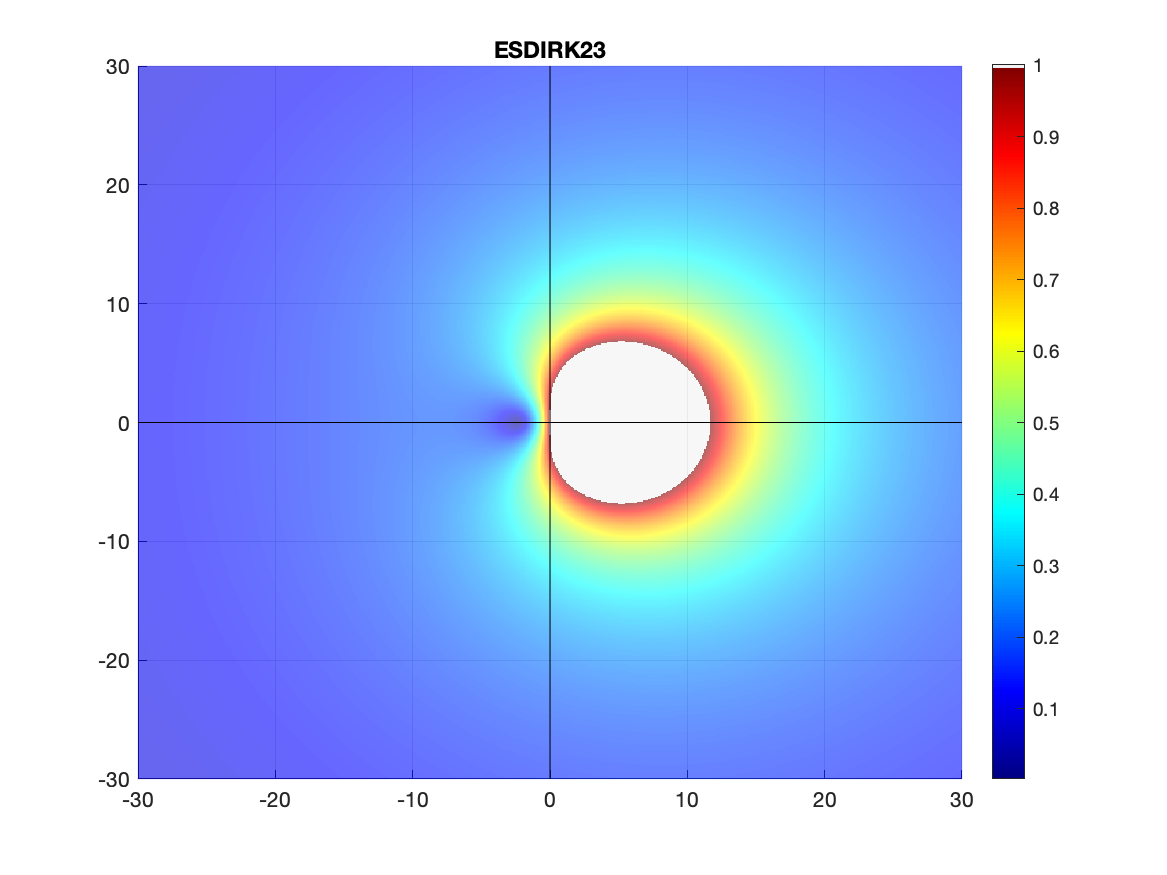
\includegraphics[width=\textwidth]{graphics/opg7/ESDIRK23-stability.png}
    \caption{Stability region of ESDIRK23, coloured area is stable}
    \label{fig7:stable}
\end{figure}

\section{Implementation of ESDIRK23 with adaptive time step}
Because ESDIRK23 is not an explicit method, we need to use an iterative method to determine each step. Specifically, we use a special form of inexact Newton, for stage 2 we want to solve

\begin{align}
    R_2(X_2) &= X_2 - h \gamma f(T_2,X_2) - \xi_2 = 0, \quad \xi_2 = x_n + h a_{21} f_1.
\end{align}
We do this by
\begin{align}
    f_2 &= f(T_2,X_2) \\
    J &= \frac{\partial f}{\partial x} (T_2,X_2) \\
    M &= I - h \gamma J \\
    M &= LU  \quad \text{LU: LU factorization of M} \\
    R_2 &= X_2 - h \gamma f(T_2,X_2) - \xi_2 \\
    LU \Delta X_2 &= -R_2 \quad \text{sole for $\Delta X_2$} \\
    X_2 :&= X_2 + \Delta X_2  \quad \text{Continue untill $||R_2|| < \varepsilon$}.
\end{align}

Notice that this is a specialized version that only works for ESDIRK23, and exploits structures in the tableau table to be more efficient.

For selecting the appropriate step size, we will use the \textit{predictive error controller} (PI controller). This means that we have

\begin{align}
    h_{n+1} &= \left ( \frac{h_n}{h_{n-1}}  \right )
    \left ( \frac{\varepsilon}{r_{n+1}} \right )^{\frac{1}{3}} 
    \left ( \frac{r_n}{r_{n+1}} \right )^{\frac{1}{3}} h_n
\end{align}
where (we use $||\cdot ||_\infty$)
\begin{align}
    r = \max_i \frac{|e_i|}{max \{AbsTol_i, |(x_n)_i| RelTol_i\} }
\end{align}

Listing \ref{lst7:esdirk} shows a Matlab implementation of a ESDIRK23 with adaptive time step.

\begin{lstlisting}[language=Matlab,caption=Implementation of ESDIRK23 with adaptive time step,label=lst7:esdirk]
function [Tout,Xout,Gout,info,stats] = ESDIRK(fun,jac,t0,tf,x0,h0,absTol,relTol,varargin)
%% ESDIRK23 Parameters 
%=========================================================================
% ESDIRK23 parameters
gamma = 1-1/sqrt(2);
a31 = (1-gamma)/2;
AT = [0 gamma a31;0 gamma a31;0 0 gamma];
c  = [0; 2*gamma; 1];
b  = AT(:,3);
bhat = [    (6*gamma-1)/(12*gamma); ...
    1/(12*gamma*(1-2*gamma)); ...
    (1-3*gamma)/(3*(1-2*gamma))    ];
d  = b-bhat;
p  = 2;
phat = 3;
s = 3;

% error and convergence controller
epsilon = 0.8;
tau = 0.1*epsilon; %0.005*epsilon;
itermax = 20;
ke0 = 1.0/phat;
ke1 = 1.0/phat;
ke2 = 1.0/phat;
alpharef = 0.3;
alphaJac = -0.2;
alphaLU  = -0.2;
hrmin = 0.01;
N = ceil((tf-t0)/hmin);
hs = zeros(2,N+1);
hrmax = 10;
%========================================================================
tspan = [t0 tf]; % carsten
info = struct(...
            'nStage',    s,       ... % carsten
            'absTol',    'dummy',  ... % carsten
            'relTol',    'dummy',  ... % carsten
            'iterMax',   itermax, ... % carsten
            'tspan',     tspan,   ... % carsten
            'nFun',      0, ...
            'nJac',      0, ...
            'nLU',       0, ...
            'nBack',     0, ...
            'nStep',     0, ...
            'nAccept',   0, ...
            'nFail',     0, ...
            'nDiverge',  0, ...
            'nSlowConv', 0);


        
%% Main ESDIRK Integrator
%========================================================================
nx = size(x0,1);
F = zeros(nx,s);
t = t0;
x = x0;
h = h0;

[F(:,1),g]  = feval(fun,t,x,varargin{:});
info.nFun = info.nFun+1;
[dfdx,dgdx] = feval(jac,t,x,varargin{:});
info.nJac = info.nJac+1;
FreshJacobian = true;
if (t+h)>tf
    h = tf-t;
end
hgamma = h*gamma;
dRdx = dgdx - hgamma*dfdx;
[L,U,pivot] = lu(dRdx,'vector');
info.nLU = info.nLU+1;
hLU = h;

FirstStep = true;
ConvergenceRestriction = false;
PreviousReject = false;
iter = zeros(1,s);

% Output
chunk = 100;
Tout = zeros(chunk,1);
Xout = zeros(chunk,nx);
Gout = zeros(chunk,nx); 

Tout(1,1) = t;
Xout(1,:) = x.';
Gout(1,:) = g.';

runs = 1;
while t<tf
    info.nStep = info.nStep+1;
    %=====================================================================
    % A step in the ESDIRK method
    i=1;   
    diverging = false;
    SlowConvergence = false; % carsten
    alpha = 0.0;
    Converged = true;
    while (i<s) && Converged
        % Stage i=2,...,s of the ESDIRK Method
        i=i+1;
        phi = g + F(:,1:i-1)*(h*AT(1:i-1,i));

        % Initial guess for the state
         if i==2
             dt = c(i)*h;
             G = g + dt*F(:,1);
             X = x + dgdx\(G-g);
         else
             dt = c(i)*h;
             G  = g + dt*F(:,1);
             X  = x + dgdx\(G-g);
         end
        T = t+dt;
            
        [F(:,i),G] = feval(fun,T,X,varargin{:});
        info.nFun = info.nFun+1;
        R = G - hgamma*F(:,i) - phi;
%        rNewton = norm(R./(absTol + abs(G).*relTol),2)/sqrt(nx);
        rNewton = norm(R./(absTol + abs(G).*relTol),inf);
        Converged = (rNewton < tau);
        %iter(i) = 0; % original, if uncomment then comment line 154: iter(:) = 0;
        % Newton Iterations
        while ~Converged && ~diverging && ~SlowConvergence%iter(i)<itermax
            iter(i) = iter(i)+1;
            dX = U\(L\(R(pivot,1)));
            info.nBack = info.nBack+1;
            X = X - dX;
            rNewtonOld = rNewton;
            [F(:,i),G] = feval(fun,T,X,varargin{:});
            info.nFun = info.nFun+1;
            R = G - hgamma*F(:,i) - phi;
%            rNewton = norm(R./(absTol + abs(G).*relTol),2)/sqrt(nx);
            rNewton = norm(R./(absTol + abs(G).*relTol),inf);
            alpha = max(alpha,rNewton/rNewtonOld);
            Converged = (rNewton < tau);
            diverging = (alpha >= 1);
            SlowConvergence = (iter(i) >= itermax); % carsten
            %SlowConvergence = (alpha >= 0.5); % carsten
            %if (iter(i) >= itermax), i, iter(i), Converged, diverging, pause, end % carsten
        end
        %diverging = (alpha >= 1); % original, if uncomment then comment line 142: diverging = (alpha >= 1)*i;
        diverging = (alpha >= 1)*i; % carsten, recording which stage is diverging
    end
    %if diverging, i, iter, pause, end
    nstep = info.nStep;
    stats.t(nstep) = t;
    stats.h(nstep) = h;
    stats.r(nstep) = NaN;
    stats.iter(nstep,:) = iter;
    stats.Converged(nstep) = Converged;
    stats.Diverged(nstep)  = diverging;
    stats.AcceptStep(nstep) = false;
    stats.SlowConv(nstep)  = SlowConvergence*i; % carsten, recording which stage is converging to slow (reaching maximum no. of iterations)
    iter(:) = 0; % carsten
    %=====================================================================
    % Error and Convergence Controller
    if Converged
        % Error estimation
        e = F*(h*d);
%        r = norm(e./(absTol + abs(G).*relTol),2)/sqrt(nx);
        r = norm(e./(absTol + abs(G).*relTol),inf);
        CurrentStepAccept = (r<=1.0);
        r = max(r,eps);
        stats.r(nstep) = r;
        % Step Length Controller
        if CurrentStepAccept
            stats.AcceptStep(nstep) = true;
            info.nAccept = info.nAccept+1;
            if FirstStep || PreviousReject || ConvergenceRestriction
                % Aymptotic step length controller
                hr = 0.75*(epsilon/r)^ke0; 
            else
                % Predictive controller
                s0 = (h/hacc);
                s1 = max(hrmin,min(hrmax,(racc/r)^ke1));
                s2 = max(hrmin,min(hrmax,(epsilon/r)^ke2));
                hr = 0.95*s0*s1*s2;
            end
            racc = r;
            hacc = h;
            FirstStep = false;
            PreviousReject = false;
            ConvergenceRestriction = false;
            
            % Next Step
            t = T;
            x = X;
            g = G;
            F(:,1) = F(:,s);            
            
        else % Reject current step
            info.nFail = info.nFail+1;
            if PreviousReject
                kest = log(r/rrej)/(log(h/hrej));
                kest = min(max(0.1,kest),phat);
                hr   = max(hrmin,min(hrmax,((epsilon/r)^(1/kest))));
            else
                hr = max(hrmin,min(hrmax,((epsilon/r)^ke0)));
            end
            rrej = r;
            hrej = h;
            PreviousReject = true;
        end
   
        % Convergence control
        halpha = (alpharef/alpha);
        if (alpha > alpharef)
            ConvergenceRestriction = true;
            if hr < halpha
                h = max(hrmin,min(hrmax,hr))*h;
            else
                h = max(hrmin,min(hrmax,halpha))*h;
            end
        else
            h = max(hrmin,min(hrmax,hr))*h;
        end
        h = max(1e-8,h);
        if (t+h) > tf
            h = tf-t;
        end
        
        % Jacobian Update Strategy
        FreshJacobian = false;
        if alpha > alphaJac
            [dfdx,dgdx] = feval(jac,t,x,varargin{:});
            info.nJac = info.nJac+1;
            FreshJacobian = true;
            hgamma = h*gamma;
            dRdx = dgdx - hgamma*dfdx; 
            [L,U,pivot] = lu(dRdx,'vector');
            info.nLU = info.nLU+1;
            hLU = h;
        elseif (abs(h-hLU)/hLU) > alphaLU 
            hgamma = h*gamma;
            dRdx = dgdx-hgamma*dfdx;
            [L,U,pivot] = lu(dRdx,'vector');
            info.nLU = info.nLU+1;
            hLU = h;
        end        
    else % not converged
        info.nFail=info.nFail+1;
        CurrentStepAccept = false;
        ConvergenceRestriction = true;
        if FreshJacobian && diverging
            h = max(0.5*hrmin,alpharef/alpha)*h;
            info.nDiverge = info.nDiverge+1;
        elseif FreshJacobian
            if alpha > alpharef
                h = max(0.5*hrmin,alpharef/alpha)*h;
            else
                h = 0.5*h;
            end
        end
        if ~FreshJacobian
            [dfdx,dgdx] = feval(jac,t,x,varargin{:});
            info.nJac = info.nJac+1;
            FreshJacobian = true;
        end
        hgamma = h*gamma;
        dRdx = dgdx - hgamma*dfdx;
        [L,U,pivot] = lu(dRdx,'vector');
        info.nLU = info.nLU+1;
        hLU = h;
    end
    
    %=====================================================================
    % Storage of variables for output
    
    if CurrentStepAccept
       nAccept = info.nAccept;
       if nAccept > length(Tout)
           Tout = [Tout; zeros(chunk,1)];
           Xout = [Xout; zeros(chunk,nx)];
           Gout = [Gout; zeros(chunk,nx)];
       end
       Tout(nAccept,1) = t;
       Xout(nAccept,:) = x.';
       Gout(nAccept,:) = g.';
    end

    
end
info.nSlowConv = length(find(stats.SlowConv)); % carsten
nAccept = info.nAccept;
Tout = Tout(1:nAccept,1);
Xout = Xout(1:nAccept,:);
Gout = Gout(1:nAccept,:);
\end{lstlisting}

\section{Test on Van der Pol problem and comparison with Matlab ODE solvers}
Now that we have an implementation of ESDIRK23 with adaptive step size we want to test it. To do so we look at the Van der Pol problem given by
\begin{align}
    \Ddot{x}(t) &= \mu (1-x(t)^2) \dot{x}(t) - x(t).
\end{align}
To solve the problem we must first re-write the problem as a system of first order differential equations. Luckily this is done easily and given by
\begin{align}
    \dot{x}_1(t) &= x_2(t) \\
    \dot{x}_2(t) &= \mu(1-x_1(t)^2) x_2(t) - x_1(t).
\end{align}

We will now test ESDIRK23 on the Van der Pol problem with $\mu = 3$ and $\mu = 20$. 

\subsection{Van der Pol, $\mu = 3$}
Figure \ref{fig7:mu3} shows the numerical solution to the Van der Pol problem with $\mu = 3$ for ESDIRK23 with adaptive time steps and $AbsTol=RelTol \in \{10^{-2}, 10^{-4}, 10^{-6}\}$, ODE45 and ODE15s. Notice also that for $Tol = 10^{-2}$ the only difference visible is again due to the relatively large steps that the algorithm takes in the "non-stiff" area. Otherwise, all tolerances seem to follow the ODE45/ODE15s solutions very well.

\begin{figure}[H]
    \centering
    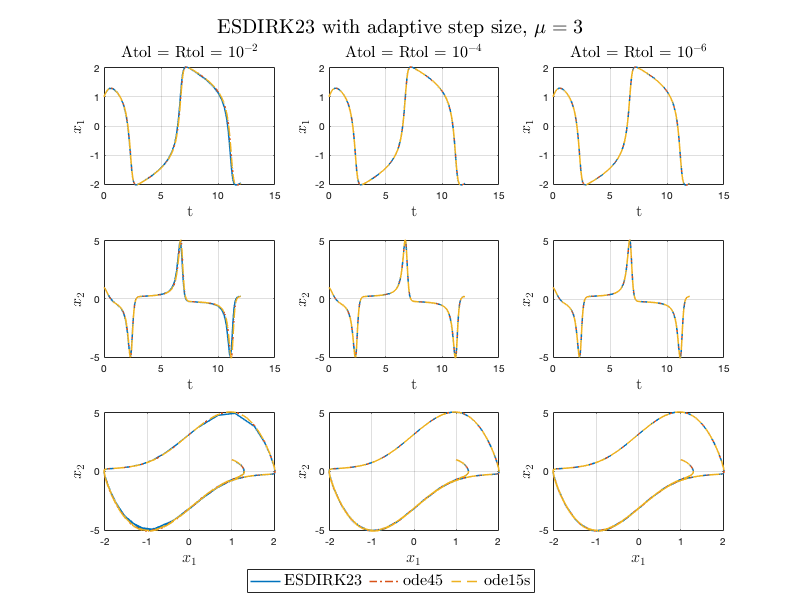
\includegraphics[width=\textwidth]{graphics/opg7/mu3.png}
    \caption{Solution to Van der Pol with $\mu = 3$ using adaptive step sizes}
    \label{fig7:mu3}
\end{figure}

Table \ref{tab7:mu3} shows the CPU time and number of function evaluations when solving the Van der Pol problem with $\mu = 3$ using different tolerances and Matlab ODE solvers. Notice that with $Tol = 10^{-2}$ the ESDIRK23 is relatively fast (slower than ODE45 but faster than ODE15s). Generally, it is very hard to tell the solutions curves apart just by looking at them. Even for the lowest tolerance, we get quite good results. What is interesting is the CPU time usage and number of function evaluations used at the different tolerances. For both explicit- and implicit Euler, we saw that the CPU time and function evaluations increased dramatically when we required higher accuracy, now this increase is not as pronounced. This demonstrates the power of higher order methods quite well.

\begin{table}[H]
    \centering
    \caption{CPU time and function evaluations of ESDIRK23 with adaptive time step and Matlab ODE solvers}
    \begin{tabular}{|c||c|c|c|c|c|c|} \hline
         \textbf{Method}    & $Tol = 10^{-2}$&   $Tol = 10^{-4}$ & $Tol = 10^{-6}$ & ODE45 & ODE15s     \\ \hline \hline 
         \textbf{Time}      & 0.0122 &   0.0167  &  0.0549 & 0.0046 & 0.0175   \\ \hline
         \textbf{Fun evals} & 517    &   1199  &    4488 & 1069 & 926  \\ \hline
    \end{tabular}
    \label{tab7:mu3}
\end{table}

Figure \ref{fig7:mu3_h} shows the used step sizes for the different tolerances. The red crosses mark whenever the step size controller failed to set the step size correctly, i.e., whenever the estimated (using the embedded error estimate) error was larger than the allowed maximum. Notice that the behaviour of all three tolerances are quite similar. Also notice that the step sizes does not vary nearly as much for the individual tolerances as previously seen (for explicit- and implicit Euler). Additionally, if we look at the difference in step sizes for the different tolerances, we see that in order to decrease the tolerance by a factor $10^4$, we do not even need to decrease the step size by a factor $10^2$. This is the true power of higher order methods! 

\begin{figure}[H]
    \centering
    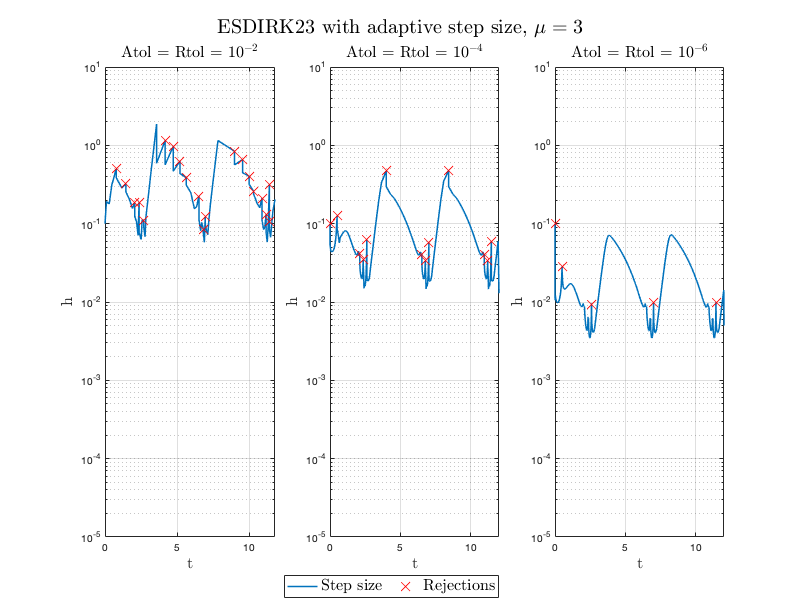
\includegraphics[width=\textwidth]{graphics/opg7/mu3_h.png}
    \caption{Step sizes when solving the Van der Pol with $\mu = 3$ at different tolerances}
    \label{fig7:mu3_h}
\end{figure}

\subsection{Van der Pol, $\mu = 20$}
The Van der Pol problem with $\mu = 20$ is a more complicated problem. The dynamics of the problem is largely defined by the $\mu$ parameter. In particular, the problem becomes more stiff when $\mu$ is increased.

Figure \ref{fig7:mu20} shows the numerical solution to the Van der Pol problem with $\mu = 20$ for ESDIRK23 with adaptive time steps and $AbsTol=RelTol \in \{10^{-2}, 10^{-4}, 10^{-6}\}$, ODE45 and ODE15s. Notice that for $Tol = 10^{-2}$ we see some difference in the plots. ESDIRK23 seem to be a bit to far \textit{ahead}, i.e., ESDIRK23 makes abrupt jump in values slightly before ODE45/ODE15s. The reason fore this is because it is to a large extend an implicit method. As such is has many characteristics of a right point method. In chapter 3, we saw the same sort of behaviour from implicit Euler.

\begin{figure}[H]
    \centering
    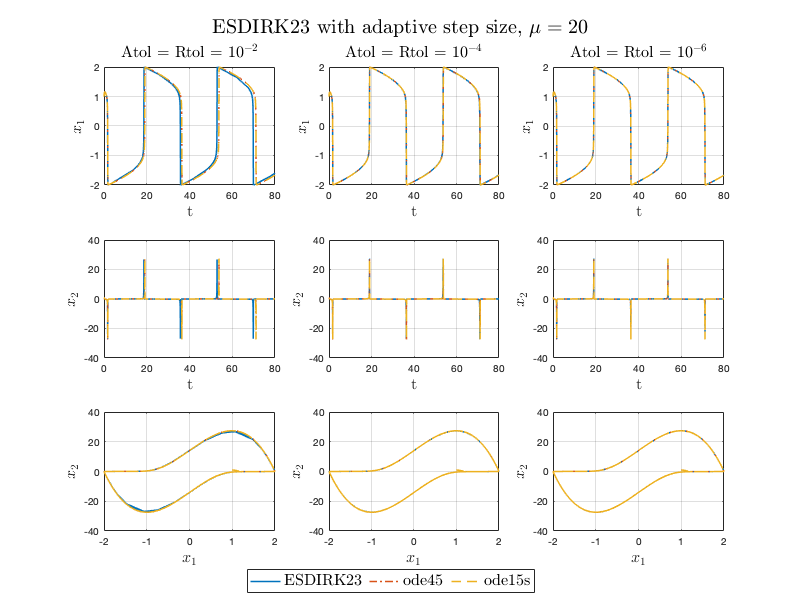
\includegraphics[width=\textwidth]{graphics/opg7/mu20.png}
    \caption{Solution to Van der Pol with $\mu = 20$ using adaptive step sizes}
    \label{fig7:mu20}
\end{figure}

Table \ref{tab7:mu20} shows that CPU time and number of function evaluations when solving the Van der Pol problem with $\mu = 20$ using different tolerances and Matlab ODE solvers. Notice that with $Tol = 10^{-2}$ the ESDIRK23 is very similar in speed to ODE45 (and faster than ODE15s). Once again notice that 100 times the accuracy does not require 100 times the CPU time or 100 times the function calls. This is because ESDIRK23 is a 2nd order method, i.e., the accuracy increase much faster than linear. 

\begin{table}[H]
    \centering
    \caption{CPU time and function evaluations of ESDIRK23 with adaptive time step and Matlab ODE solvers}
    \begin{tabular}{|c||c|c|c|c|c|c|} \hline
         \textbf{Method}    & $Tol = 10^{-2}$&   $Tol = 10^{-4}$ & $Tol = 10^{-6}$ & ODE45 & ODE15s     \\ \hline \hline 
         \textbf{Time}      & 0.0317   & 0.0445  &   0.1558 & 0.0386 & 0.0612   \\ \hline
         \textbf{Fun evals} &  1384     &   3383    &   12560 & 8461 & 2944  \\ \hline
    \end{tabular}
    \label{tab7:mu20}
\end{table}

Figure \ref{fig7:mu20_h} shows the used step sizes for the different tolerances. The red crosses mark whenever the step size controller failed to set the step size correctly, i.e., whenever the estimated error was larger than the allowed maximum. Notice that the behaviour of all three tolerances are not nearly as similar as previously seen. Notice that the step sizes does not vary nearly as much for the individual tolerances as previously seen (for explicit- and implicit Euler). In fact, we see that for a difference of a factor $10^4$ in accuracy, the difference is approximate a factor $10^2$ in step size. This is consistent with ESDIRK23 being a 2nd order method. 

\begin{figure}[H]
    \centering
    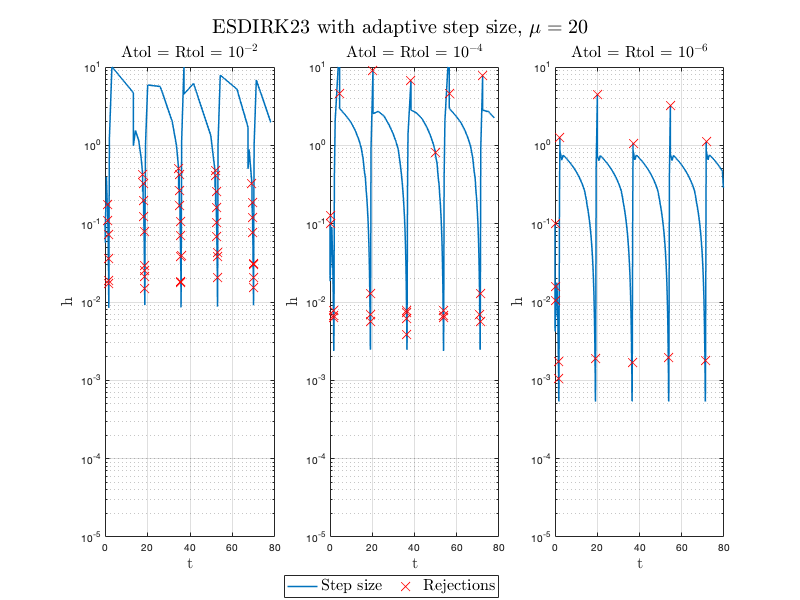
\includegraphics[width=\textwidth]{graphics/opg7/mu20_h.png}
    \caption{Step sizes when solving the Van der Pol with $\mu = 20$ at different tolerances}
    \label{fig7:mu20_h}
\end{figure}

